\documentclass[11pt,]{article}
\usepackage{lmodern}
\usepackage{amssymb,amsmath}
\usepackage{ifxetex,ifluatex}
\usepackage{fixltx2e} % provides \textsubscript
\ifnum 0\ifxetex 1\fi\ifluatex 1\fi=0 % if pdftex
  \usepackage[T1]{fontenc}
  \usepackage[utf8]{inputenc}
\else % if luatex or xelatex
  \ifxetex
    \usepackage{mathspec}
  \else
    \usepackage{fontspec}
  \fi
  \defaultfontfeatures{Ligatures=TeX,Scale=MatchLowercase}
\fi
% use upquote if available, for straight quotes in verbatim environments
\IfFileExists{upquote.sty}{\usepackage{upquote}}{}
% use microtype if available
\IfFileExists{microtype.sty}{%
\usepackage{microtype}
\UseMicrotypeSet[protrusion]{basicmath} % disable protrusion for tt fonts
}{}
\usepackage[margin=1in]{geometry}
\usepackage{hyperref}
\PassOptionsToPackage{usenames,dvipsnames}{color} % color is loaded by hyperref
\hypersetup{unicode=true,
            pdftitle={Mapping Environmental Action in Scotland},
            pdfauthor={Jeremy H. Kidwell},
            colorlinks=true,
            linkcolor=black,
            citecolor=Blue,
            urlcolor=Blue,
            breaklinks=true}
\urlstyle{same}  % don't use monospace font for urls
\usepackage{natbib}
\bibliographystyle{plainnat}
\usepackage{longtable,booktabs}
\usepackage{graphicx,grffile}
\makeatletter
\def\maxwidth{\ifdim\Gin@nat@width>\linewidth\linewidth\else\Gin@nat@width\fi}
\def\maxheight{\ifdim\Gin@nat@height>\textheight\textheight\else\Gin@nat@height\fi}
\makeatother
% Scale images if necessary, so that they will not overflow the page
% margins by default, and it is still possible to overwrite the defaults
% using explicit options in \includegraphics[width, height, ...]{}
\setkeys{Gin}{width=\maxwidth,height=\maxheight,keepaspectratio}
\IfFileExists{parskip.sty}{%
\usepackage{parskip}
}{% else
\setlength{\parindent}{0pt}
\setlength{\parskip}{6pt plus 2pt minus 1pt}
}
\setlength{\emergencystretch}{3em}  % prevent overfull lines
\providecommand{\tightlist}{%
  \setlength{\itemsep}{0pt}\setlength{\parskip}{0pt}}
\setcounter{secnumdepth}{5}
% Redefines (sub)paragraphs to behave more like sections
\ifx\paragraph\undefined\else
\let\oldparagraph\paragraph
\renewcommand{\paragraph}[1]{\oldparagraph{#1}\mbox{}}
\fi
\ifx\subparagraph\undefined\else
\let\oldsubparagraph\subparagraph
\renewcommand{\subparagraph}[1]{\oldsubparagraph{#1}\mbox{}}
\fi

%%% Use protect on footnotes to avoid problems with footnotes in titles
\let\rmarkdownfootnote\footnote%
\def\footnote{\protect\rmarkdownfootnote}

%%% Change title format to be more compact
\usepackage{titling}

% Create subtitle command for use in maketitle
\newcommand{\subtitle}[1]{
  \posttitle{
    \begin{center}\large#1\end{center}
    }
}

\setlength{\droptitle}{-2em}

  \title{Mapping Environmental Action in Scotland}
    \pretitle{\vspace{\droptitle}\centering\huge}
  \posttitle{\par}
    \author{\href{http://jeremykidwell.info}{Jeremy H. Kidwell}}
    \preauthor{\centering\large\emph}
  \postauthor{\par}
      \predate{\centering\large\emph}
  \postdate{\par}
    \date{2019-02-01}


\begin{document}
\maketitle

\hypertarget{introduction15541312}{%
\section[Introduction]{\texorpdfstring{Introduction\footnote{This
  research was jointly funded by the AHRC/ESRC under project numnbers
  AH/K005456/1 and AH/P005063/1.}}{Introduction}}\label{introduction15541312}}

Until recently, environmentalism has been treated by governments and
environmental charities as a largely secular concern. In spite of the
well-developed tradition of ``eco-theology'' which began in earnest in
the UK in the mid-twentieth century (and which has many precursors in
previous centuries), third-sector groups and governments, particularly
in Britain and Europe, have largely ignored religious groups as they
have gone about their business crafting agendas for behaviour change,
developing funding programmes, and developing platforms to mitigate
ecological harm, motivate consumers and create regulation regimes. That
this has changed is evidenced by the fact that several prominent
non-religious environmental groups have commissioned studies and crafted
outreach programmes to persons with a particular faith tradition or to
``spiritual communities'' including RSPB (2013) and the Sierra Club USA
(2008).\footnote{This is not to say that there have been no
  collaborations before 2000, noteworthy in this respect is the WWF who
  helped to found the Alliance of Religion and Conservation (ARC) in
  1985.} Further, since 2008, the Scottish Government has provided a
significant portion of funding for the ecumenical charity,
Eco-Congregation Scotland, which works to promote literacy on
environmental issues in religious communities in Scotland and helps to
certify congregations under their award programme. What is not well
known, however, even by these religious environmental groups themselves,
is whether or how their membership might be different from other
environmental groups. This study represents an attempt to illuminate
this new interest with some more concrete data about religious groups in
Scotland and how they may differ from non-religious counterparts.

\hypertarget{eco-congregation-scotland-the-basics}{%
\section{Eco-Congregation Scotland: The
Basics}\label{eco-congregation-scotland-the-basics}}

There are 344 eco-congregations in Scotland. By some measurements,
particularly in terms of individual sites and possibly also with regards
to volunteers, this makes Eco-Congregation Scotland one of the largest
environmental third-sector groups in Scotland.\footnote{This suggestion
  should be qualified - RSPB would greatly exceed ECS both in terms of
  the number of individual subscribers and budget. The RSPB trustee's
  report for 2013-2014 suggests that their member base was 1,114,938
  people across Britain with a net income of £127m - the latter of which
  exceeds the Church of Scotland. If we adjust this based on the
  Scottish share of the population of the United Kingdom as of the 2011
  census (8.3\%) this leaves us with an income of £9.93m. The British
  charity commission requires charities to self-report the number of
  volunteers and staff, and from their most recent statistics we learn
  that RSPB engaged with 17,600 volunteers and employed 2,110 members of
  staff. Again, adjusted for population, this leaves 1,460 volunteers in
  Scotland and 176 staff. However, if we measure environmental groups
  based on the number of sites they maintain, RSPB has only 40 reserves
  with varying levels of local community engagement. For comparison, as
  of Sep 14 2015, Friends of the Earth Scotland had only 10 local groups
  (concentrated mostly in large urban areas). Depending on how one
  measures ``volunteerism,'' it may be possible that ECS has more
  engaged volunteers in Scotland as well - if each ECS group had only 4
  ``volunteers'' then this would exceed RSPB.}

In seeking to conduct GIS and statistical analysis of ECS, it is
important to note that there some ways in which these sites are
statistically opaque. Our research conducted through interviews at a
sampling of sites and analysis of a variety of documents suggests that
there is a high level of diversity both in terms of the number of those
participating in environmental action and the types of action underway
at specific sites. Work at a particular site can also ebb and flow over
the course of time. Of course, as research into other forms of activism
and secular environmental NGOs has shown, this is no different from any
other third sector volunteer group. Variability is a regular feature of
groups involved in activism and/or environmental concern.

For the sake of this analysis, we took each Eco-Congregation Scotland
site to represent a point of analysis as if each specific site
represented a community group which had ``opted-in'' on environmental
concern. On this basis, in this section, in the tradition of human
geography, we ``map'' environmental action among religious communities
in Scotland a variety of ways. This is the first major geographical
analysis of this kind conducted to date in Europe. We measure the
frequency and location of ECS sites against a variety of standard
geo-referenced statistical data sets, seeking to provide a statistical
and geographically based assessment of the participation of religious
groups in relation to the following:

\begin{itemize}
\tightlist
\item
  Location within Scotland
\item
  Religious affiliation
\item
  Relation to the Scottish Index of Multiple Deprivation (SIMD)
\item
  Relation to the 8-Fold Scottish Government Urban-Rural Scale
\item
  Proximity to ``wilderness'' (based on several different designations)
\end{itemize}

For the sake of comparison, we also measured the geographical footprint
of two other forms of community group in Scotland, (1) Transition Towns
(taking into account their recent merge with Scotland Communities
Climate Action Network) and (2) member groups of the Development Trust
Association Scotland (``DTAS''). These two groups provide a helpful
basis for comparison as they are not centralised and thus have a
significant geographical dispersion across Scotland. They also provide a
useful comparison as transition is a (mostly) non-religious
environmental movement, and community development trusts are not
explicitly linked to environmental conservation (though this is often
part of their remit), so we have a non-religious point of comparison in
Transition and a non-environmental point of comparison with DTAS

\hypertarget{technical-background}{%
\section{Technical Background}\label{technical-background}}

Analysis was conducted using QGIS 2.8 and R 3.5.2, and data-sets were
generated in CSV format.\footnote{Kidwell, Jeremy. (2016).
  Eco-Congregation Scotland, 2014-2016. University of Edinburgh.
  \url{http://dx.doi.org/10.7488/ds/1357}.} To begin with, I assembled a
data set consisting of x and y coordinates for each congregation in
Scotland and collated this against a variety of other specific data.
Coordinates were checked by matching UK postcodes of individual
congregations against geo-referencing data in the Office for National
Statistics postcode database. In certain instances a single
``congregation'' is actually a series of sites which have joined
together under one administrative unit. In these cases, each site was
treated as a separate data point if worship was held at that site at
least once a month, but all joined sites shared a single unique
identifier. As noted above, two other datasets were generated for the
sake of comparative analysis.\footnote{For further detail on Dataset
  generation, see Kidwell, Forthcoming, 2018.} These included one
similar Environmental Non-Governmental Organisation (ENGO) in Scotland
(1) Transition Scotland (which includes Scotland Communities Climate
Action Network);\footnote{My dataset on transition towns will be made
  available later in 2016. Initial data was aquired from the Transition
  Scotland website
  \url{http://www.transitionscotland.org/transition-in-scotland} on
  December 10, 2014. We are currently in the process of collaboratively
  generating a more up-to-date dataset which will reflect their
  collaboration with SCCAN.} and another community-based NGO, Scottish
Community Development Trusts.\footnote{Data was acquired from the
  Development Trusts Association website,
  \url{http://www.dtascot.org.uk}, accessed on 20 July 2015. As above,
  we are currently in the process of active collaboration with
  volunteers from the DTAS to co-generate a new dataset.} As this report
will detail, these three overlap in certain instances both literally and
in terms of their aims, but each also has a separate identity and
footprint in Scotland. Finally, in order to normalise data, we utilised
the PointX POI dataset which maintains a complete database of Places of
Worship in Scotland.\footnote{PointX data for ``Landscape Data'' items
  is sourced from Ordnance Survey Land-Line and MasterMap(R) and the
  data points are augmented with additional information provided through
  research by PointX staff, and data aquired from unidentified ``local
  data companie(s)'' and the ``118 Information'' database (see:
  \url{http://www.118information.co.uk}). This data is under license and
  cannot be made available for use. It is important to note that I
  became aware of inaccuracies in this dataset over the course of use
  and subsequently generated my own dataset in collaboration with
  churches in Scotland. This will be made available later in 2016. I am
  in active conversation with OS about improving the quality of the data
  in PointX regarding places of worship.}

\hypertarget{background-and-history-of-eco-congregation-scotland}{%
\section{Background and History of Eco-Congregation
Scotland}\label{background-and-history-of-eco-congregation-scotland}}

Eco-Congregation Scotland began a year before the official launch of
Eco-Congregation England and Wales, in 1999, as part of an effort by
Kippen Environment Centre (later renamed to Forth Environment Link, or
``FEL'') a charity devoted to environmental education in central
Scotland\footnote{From \url{http://www.forthenvironmentlink.org},
  accessed 12 July 2015.} to broaden the scope of its environmental
outreach to churches in central Scotland.\footnote{Interview with
  Margaret Warnock, 29 Aug 2014.} Initial funding was provided, through
Kippen Environment Centre by way of a ``sustainable action grant'' (with
funds drawn from a government landfill tax) through a government
programme called Keep Scotland Beautiful (the Scottish cousin of Keep
Britain Tidy). After this initial pilot project concluded, the Church of
Scotland provided additional funding for the project in the form of
staff time and office space. Additional funding a few years later from
the Scottish Government helped subsidise the position of a business
manager, and in 2011 the United Reformed Church contributed additional
funding which subsidised the position of a full-time environmental
chaplain for a 5-year term, bringing the total staff to five.

The programme launched officially in 2001 at Dunblane Cathedral in
Stirling and by 2005 the project had 89 congregations registered to be a
part of the programme and 25 which had completed the curriculum
successfully and received an Eco-Congregation award. By 2011, the number
of registrations had tripled to 269 and the number of awarded
congregations had quadrupled to
\texttt{sum(ecs\$award1\ \textless{}\ "01/01/2012",\ na.rm=TRUE)}. This
process of taking registrations and using a tiered award or recognition
scheme is common to many voluntary organisations. The ECS curriculum was
developed in part by consulting the Eco-Congregation England and Wales
materials which had been released just a year earlier in 1999, though it
has been subsequently revised, particularly with a major redesign in
2010. In the USA, a number of similar groups take a similar approach
including Earth Ministry (earthministry.org) and Green Faith
(greenfaith.org).

In the case of Eco-Congregation Scotland, congregations are invited to
begin by ``registering'' their interest in the programme by completing a
basic one-sided form. The next step requires the completion of an award
application, which includes a facilitated curriculum called a ``church
check-up'' and after an application is submitted, the site is visited
and assessed by third-party volunteer assessors. Sites are invited to
complete additional applications for further awards which are
incremental (as is the application process). Transition communities, at
least in the period reflected on their map, go through a similar process
(though this does not involve the use of a supplied curriculum) by which
they are marked first as ``interested,'' become ``active'' and then gain
``official'' status.\footnote{From the Transition map key, ``Green pins
  are `official' groups Blue pins are active communities who are
  connected to the Scottish Transition network Yellow pins show interest
  in this area''}

\hypertarget{representation-by-regional-authorities-council-areas}{%
\section{Representation by Regional Authorities (Council
Areas)}\label{representation-by-regional-authorities-council-areas}}

Perhaps the first important question to ask of these groups is, where
are they? I calculated the spread of eco-congregations and transition
groups across each of the 32 council areas in Scotland. Every council
area in Scotland has at least one eco-congregation or transition group).
The most are located in , with 48, whereas the mean among all the 32
council areas is 10.75, with a median of 8, standard deviation of
9.4698162, and interquartile range of 11.5. The following choropleth
maps show the relative concentration of eco-congregations (indicated by
yellow to red).

(\emph{TODO: need to implement}) Though there are too few
eco-congregations and transition groups for a numerically significant
representation in any of the intermediate geographies, mapping the
concentration of sites by agricultural parishes allows for a more
granular visual and I include this for comparison sake. Note, for the
sake of a more accurate visual communication, we have also marked out
areas of Scotland that are uninhabited with hash marks on the map of
agricultural parishes. (\emph{TODO: this will be done in the final
draft, once I get my image masking fixed!}).\footnote{This was
  calculated by calculating a 10m wide footprint for every postcode in
  Scotland, areas which are not within 10m of a postcode (as of May
  2014) are counted as uninhabited.}

\begin{figure}
\centering
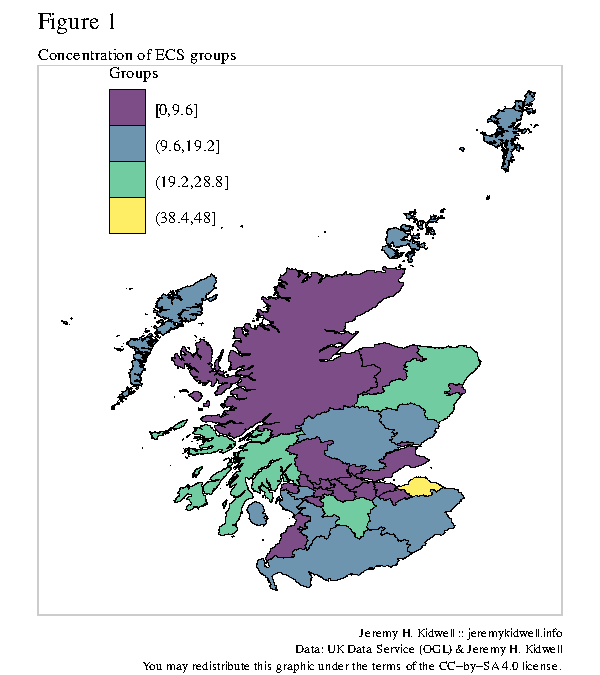
\includegraphics{figures/plot_admin_ecs_choropleth-1.pdf}
\caption{Figure 1}
\end{figure}

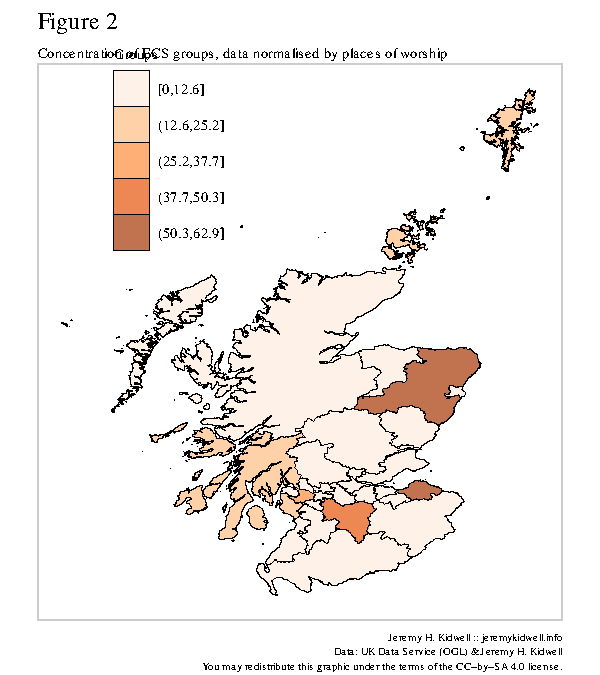
\includegraphics{figures/plot_admin_ecs_normed_choropleth-1.pdf}
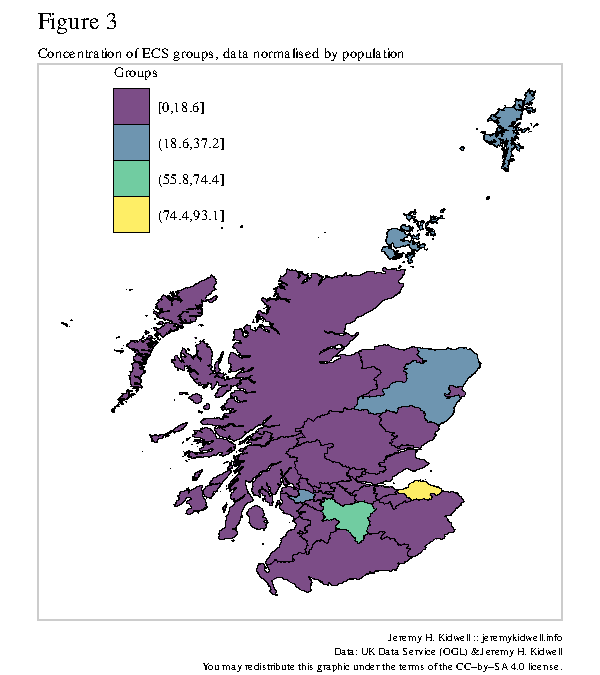
\includegraphics{figures/plot_admin_ecs_normed_choropleth-2.pdf}

Given the way population and places of worship are unevenly distributed
across Scotland it is important to represent data in terms of relative
distribution. For this study, we attempted to ``normalise'' our data in
two different ways, (1) as shown by Figure 2 above, by taking population
figures from the 2011 census (see data sheet in Appendix A) and (2) by
adjusting relative to the number of places of worship in each council
region.\footnote{See note above regarding the data used from the PointX
  POI database. Note, for our research,we filtered out religious groups
  not represented within the Eco-Congregation footprint. We discuss
  representation by tradition and religion further below.adition and
  religion further below.} The latter of these two can yield
particularly unexpected results. Thus, of the 4048 ``places of worship''
in Scotland, the highest concentration is actually the region, with 435,
second is 329 (). Rank of Council Areas by population and number of
places of worship is also included in Appendix A.

We can use this data to normalise our figures regarding Eco-Congregation
Scotland communities and this draws the presence in Edinburgh of ECS
communities into even sharper relief, as Edinburgh, though ranked second
in terms of population and fifth in terms of places of worship, ranks
first for the presence of all ECS congregations and awarded ECS
congregations. However, taking population as the basis for normalisation
first, we find that Edinburgh is far from the most prominent outlier. In
trying to communicate this difference for a lay-audience, we have chosen
to list this difference as a multiplier (i.e.~there are 2.x times as
many congregations as their share of population and an average figure of
congregations might allow for) as this conveys the difference in a
straight-forward way. Outliers where the disparity between their
relative share of the total ECS footprint and their relative share of
population is different by a positive ratio of more than double include
the Orkney Islands (3.7 times more eco-congregations than their expected
average share based on population), Argyll and Bute
(\texttt{admin\_lev1{[}CODE=S12000023{]}\$ecs\_pop\_factor} 4.2x),
Stirling (2.76x), and Perthshire and Kinross (2.18x). Interestingly,
there are no outliers whose relative share of the total footprint of ECS
is double or more in the negative direction (see Appendix A chart for
full numbers).

Turning to the total of 4048 ``places of worship'' in Scotland, we find
a slightly different picture of the relative concentration of
Eco-Congregations in Scotland. In this case, the outliers are

Whereas our initial measurements indicated a prominent lead for
Edinburgh, by normalising our data in this way we can highlight the
stronger-than-expected presence of several others that might otherwise
escape notice because they lie in a region with significantly lower
population or numerically less places of worship. Taking the PointX data
on ``places of worship'' in Scotland, we find a less dramatic picture,
but also a slightly different one. The positive outliers include East
Renfrewshire (3.4x) Edinburgh (2.9x), Stirling (2.2), West Lothian
(1.9x) and Aberdeen (1.5x). Again, negative outliers are far less
dramatic, with only Midlothian possessing a ratio of more than 100\%
negative difference from the number of ``places of worship'' at 1.5x
\emph{fewer}.

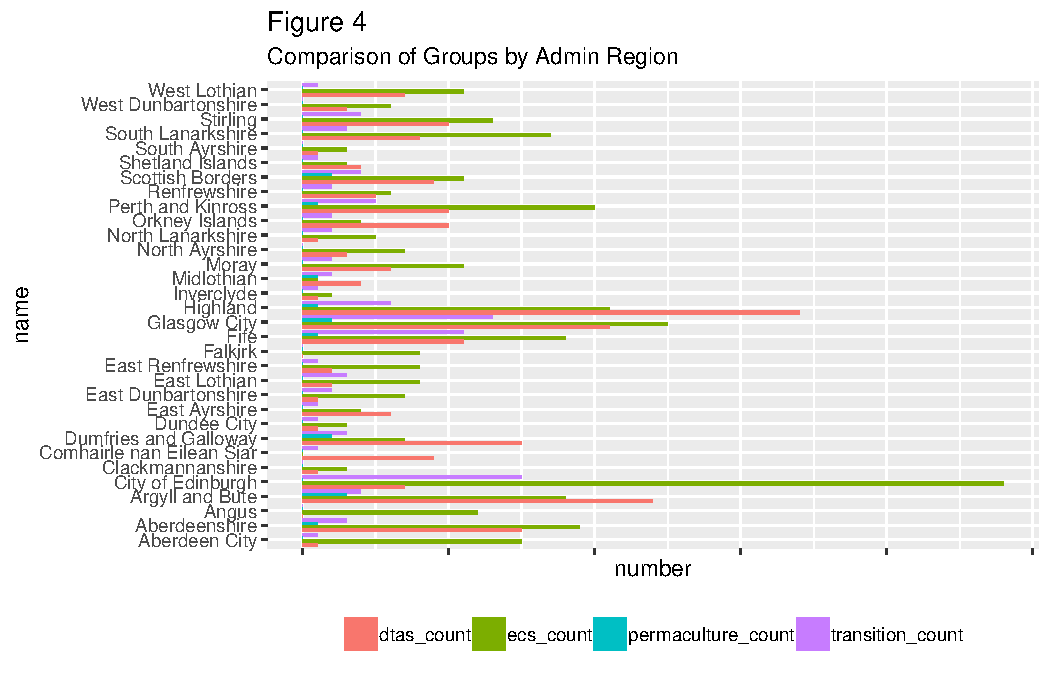
\includegraphics{figures/create_admin_barplot-1.pdf}

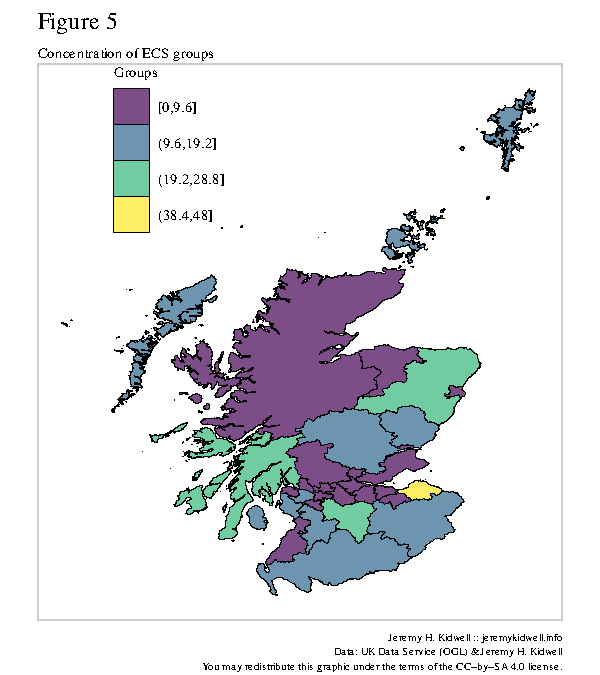
\includegraphics{figures/create_choropleth_others-1.pdf}
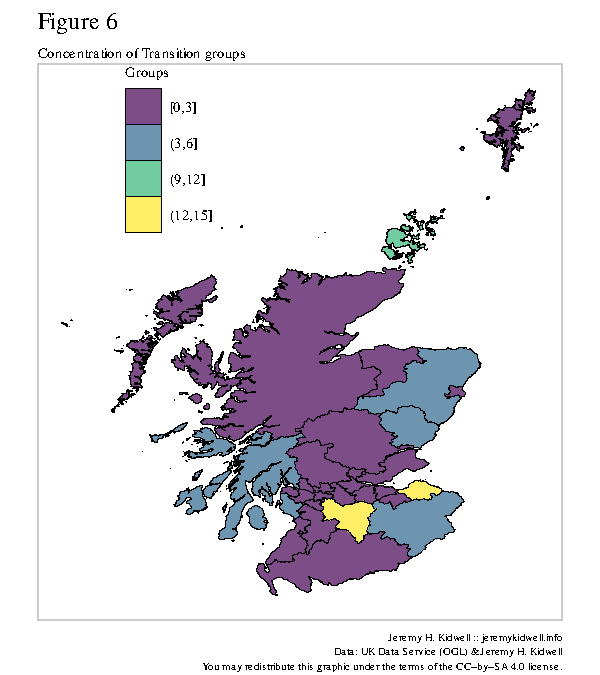
\includegraphics{figures/create_choropleth_others-2.pdf}
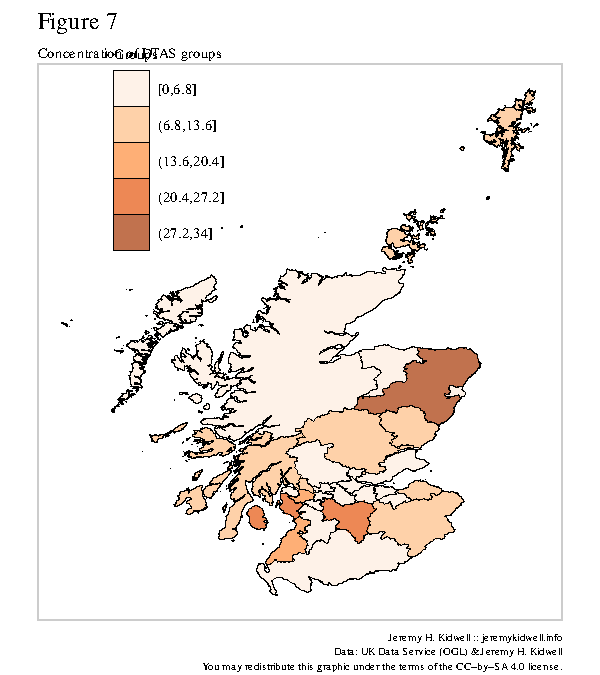
\includegraphics{figures/create_choropleth_others-3.pdf}

We can compare the representation in these various regions against our
comparison groups to see how other community-based organisations cluster
in Scottish administrative districts. Here there are some significant
contrasts. Scottish Community Development trusts are most intensely
concentrated in the Highlands and Argyll \& Bute. But, this is
consistent with all the other categories, Eco-Congregations, Places of
Worship, and dtas are all over-represented in this area, varying only by
the degree. Edinburgh is different, here we find that Eco-Congregations
and Transition projects are over-represented, while dtass are
under-represented. Finally, the highlands are another strong contrast,
here we find a very strong over-representation by transition towns and
dtass while the representation of Eco-Congregations is relatively close
to the population share for that area. The two areas of greatest
contrast for Eco-Congregations from the other groups are unsurprising,
Edinburgh is the location of the ECS offices, while Stirling is the area
in which ECS first began (see Appendix B for full data).

\hypertarget{christian-denominations}{%
\section{Christian Denominations}\label{christian-denominations}}

Eco-Congregation Scotland describes itself as an ``ecumenical movement
helping local groups of Christians link environmental issues to their
faith, reduce their environmental impact and engage with their local
community.'' There are several ties to the Church of Scotland, as the
denomination provides office space to Eco-Congregation Scotland in the
Church of Scotland complex at 121 George Street in Edinburgh and
provides funding for one full-time member of staff. In spite of this,
ECS has, from the start, attempted to emphasise its ecumenical
aspirations and this is reflected in a wide variety of ways. The name
``eco-congregation'' is meant to be tradition neutral (in interviews,
staff noted how they have sought to avoid names such as ``eco-kirk''
which would be the more obvious Presbyterian title, or ``eco-community''
or ``eco-church'' which might indicate allegiance towards another).
Further, the group has a environmental chaplain on their staff whose
position is funded by the United Reformed Church, and other members of
staff are funded by the Scottish government, and as such, carry no
formal affiliation with a religious institution. This diversity and
ecumenicism is reflected in a membership which is, though dominated by
the Church of Scotland, nevertheless, made up of a range of Christian
traditions.

Though these are not numerically significant, it is important to note
that some member congregations describe themselves as ecumenical
communities, and others are hybrids reflecting the merging of two
traditions. As this ecumenical/hybrid designation involves a small
number of the overall total, for the sake of this research, these have
been combined into a category called ``ecumenical.'' Further, as
research conducted by Church of Scotland statistician Fiona Tweedie has
shown, in many Scottish communities with only one church, members of
this church will specify their denominational affiliation in a variety
of ways (Roman Catholic, Quaker, Methodist, etc.) even though the church
and its minister are formally affiliated with the Church of
Scotland.\footnote{Fiona Tweedia, \emph{Ecumenical Audit: Questionnaire
  Findings} (2014).} So, we should be careful not to assume that the
various denominational affiliations of eco-congregations are indicative
in an absolute way.

A wide variety of historians and sociologists of religion have noted the
regional significance of different Christian denominations in Scotland
so we sought to assess the relative distribution and concentration of
eco-congregations by denomination. Finding comparative statistics is a
complex task, made more complicated by several factors. First, most
demographic data on religious belonging in Scotland comes in the form of
the 2011 census and as such is far more atomised than this data-set
which identifies groups at the level of ``congregations'' rather than
individuals. Equating these two is also complex, as participation by
members of congregations can be measured in a variety of ways, there are
often a small number of active participants in each eco-congregation
group, but may also be a large scale, but passive, support by the wider
community.

So why provide this kind of data (i.e.~at the level of individual
churches) when more granular data (i.e.~at the level of individuals
persons) is available in the form of the census and related parallel
publications such as the 2008 Scottish Environmental Attitudes survey?
We believe that mapping places of worship provides a useful intermediate
level of analysis and may complement our more atomised understanding of
EA which has been assessed at the level of individual persons to date.
Because representation within some administrative areas of Scotland, can
lead to a small number of data points, we have kept analysis to a
National level and have not provided more specific administrative-area
level calculations.

\begin{longtable}[]{@{}lr@{}}
\caption{ECS by denomination}\tabularnewline
\toprule
& x\tabularnewline
\midrule
\endfirsthead
\toprule
& x\tabularnewline
\midrule
\endhead
Baptist & 4\tabularnewline
C of S & 254\tabularnewline
C of S / URC & 3\tabularnewline
Cong & 1\tabularnewline
Ecu & 5\tabularnewline
FCS & 1\tabularnewline
Independent & 2\tabularnewline
Meth & 4\tabularnewline
Non. & 1\tabularnewline
Quaker & 1\tabularnewline
RC & 15\tabularnewline
SEC & 41\tabularnewline
Unitarian & 1\tabularnewline
URC & 11\tabularnewline
\bottomrule
\end{longtable}

As one might expect, there is a strong representation of the Church of
Scotland, almost 74\% of eco-congregations, with this number remaining
the same when we only count awarded sites. We can confirm, on the basis
of this analysis that ECS has a disproportional representation by Church
of Scotland churches. At the 2002 church census count, it only
represented 40.20\% of Scottish churches (1666 of 4144 total churches).
Similarly, on the 2011 Scottish census, only 32.44\% of persons claimed
to be members of the Church of Scotland. We can adjust this
representation to 60\%, if one excludes the 2,445,204 persons (46\% of
the total on the census) who reported either ``no religion'' or
adherence to a religious tradition not currently represented among the
eco-congregation sites. There is a slight over-representation by the
United Reformed church, though this seems considerably more dramatic
when one takes into account the fact that this is a trebling or more of
their overall share of Scottish churches. The URC makes up only sightly
more than 1\% of church buildings in Scotland and a tiny 0.04\% of
respondents to the 2011 census. The Scottish Episcopal church hovers
right around a proportional representation within ECS. More concerning
are the significant underrepresentation by Roman Catholic churches,
Baptists, the Free Church of Scotland, and other independent churches.

While Roman Catholic churches make up just over 10\% of the church
buildings in Scotland, less than 5\% of churches registered as
eco-congregations are RC. Even more dramatic is the quartering of
baptist churches, and the non-existent representation among the
significant group of independent churches and small denominations. These
make up nearly 25\% of all Scottish churches (over a thousand) and yet
only 4 have registered as eco-congregations. We provide several
tentative advisories in response to these under-representations in the
final section of this paper.

\hypertarget{eco-congregations-urban-rural-and-remote}{%
\section{Eco-Congregations, Urban, Rural and
Remote}\label{eco-congregations-urban-rural-and-remote}}

\begin{verbatim}
## OGR data source with driver: ESRI Shapefile 
## Source: "/Users/jeremy/gits/mapping_environmental_action/data", layer: "SG_UrbanRural_2016"
## with 8 features
## It has 6 fields
\end{verbatim}

Rather than bifurcate congregations into an urban/rural dichotomy, for
this study we used the Scottish Government's six-point remoteness scale
to categorise eco-congregations along a spectrum of highly populated to
remote areas. This 8-fold scale (calculated biennially) offers a more
nuanced measurement that combines measurements of remoteness and
population along the following lines:

\begin{enumerate}
\def\labelenumi{\arabic{enumi}.}
\tightlist
\item
  Large Urban Areas - Settlements of over 125,000 people.
\item
  Other Urban Areas - Settlements of 10,000 to 125,000 people.
\item
  Accessible Small Towns - Settlements of between 3,000 and 10,000
  people, and within a 30 minute drive time of a Settlement of 10,000 or
  more.
\item
  Remote Small Towns - Settlements of between 3,000 and 10,000 people,
  and with a drive time between 30 and 60 minutes to a Settlement of
  10,000 or more.
\item
  Very Remote Small Towns - Settlements of between 3,000 and 10,000
  people, and with a drive time of over 60 minutes to a Settlement of
  10,000 or more.
\item
  Accessible Rural Areas - Areas with a population of less than 3,000
  people, and within a drive time of 30 minutes to a Settlement of
  10,000 or more.
\item
  Remote Rural Areas - Areas with a population of less than 3,000
  people, and with a drive time of between 30 and 60 minutes to a
  Settlement of 10,000 or more.
\item
  Very Remote Rural Areas - Areas with a population of less than 3,000
  people, and with a drive time of over 60 minutes to a Settlement of
  10,000 or more.
\end{enumerate}

The key question which this analysis seeks to answer is whether ECS, or
the other groups surveyed, are more concentrated in Urban or Rural
areas, so as is the case below with our analysis of deprivation, we are
concerned with the outer conditions, i.e.~the urban areas (items 1-2)
and remote areas (items 7-8).

Of all the groups surveyed in this study, Eco-Congregation Scotland is
the most heavily concentrated in large urban areas (33.53\%), exceeding
by almost 50\% the rate for all places of worship (22.96\% in large
urban areas). Transition is a much more modest 20\% and development
trusts a bit lower at 15\%. It is interesting to note that the rate of
ECS concentration in these large urban areas matches the level of
overall population distribution (34.5\%). On the other end of the scale,
Eco-Congregation Scotland is the least concentrated in remote rural
areas (with 3.93\% on level 7 and 5.44\% on level 8 on the urban-rural
scale), though again, they correlate roughly to the general population
distribution (3.2\% and 2.9\% respectively). Places of worship outpace
both the population of Scotland and the footprint of Eco-Congregation
Scotland, with 14.98\% in very remote rural areas, but this is exceeded
by transition at 16.47\% and both by Scottish community development
trusts at 32.14\%. So while Eco-Congregation Scotland correlates roughly
with Scottish population distribution across the urban-rural scale, it
has a considerably more urban profile than either of the other two
groups surveyed.

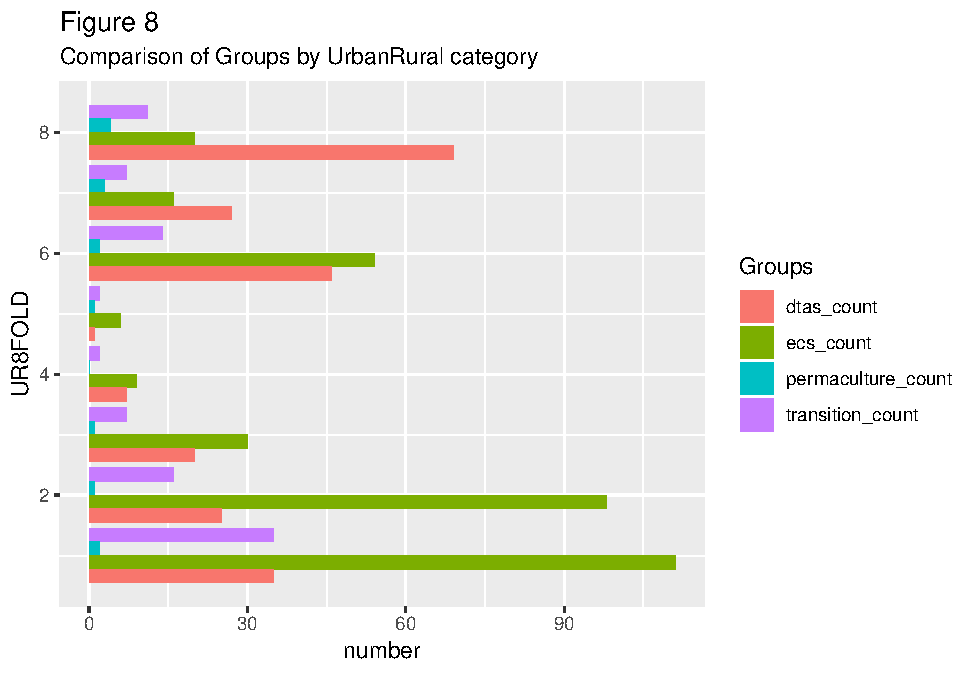
\includegraphics{figures/create_ur_barplot-1.pdf}

\begin{figure}
\centering
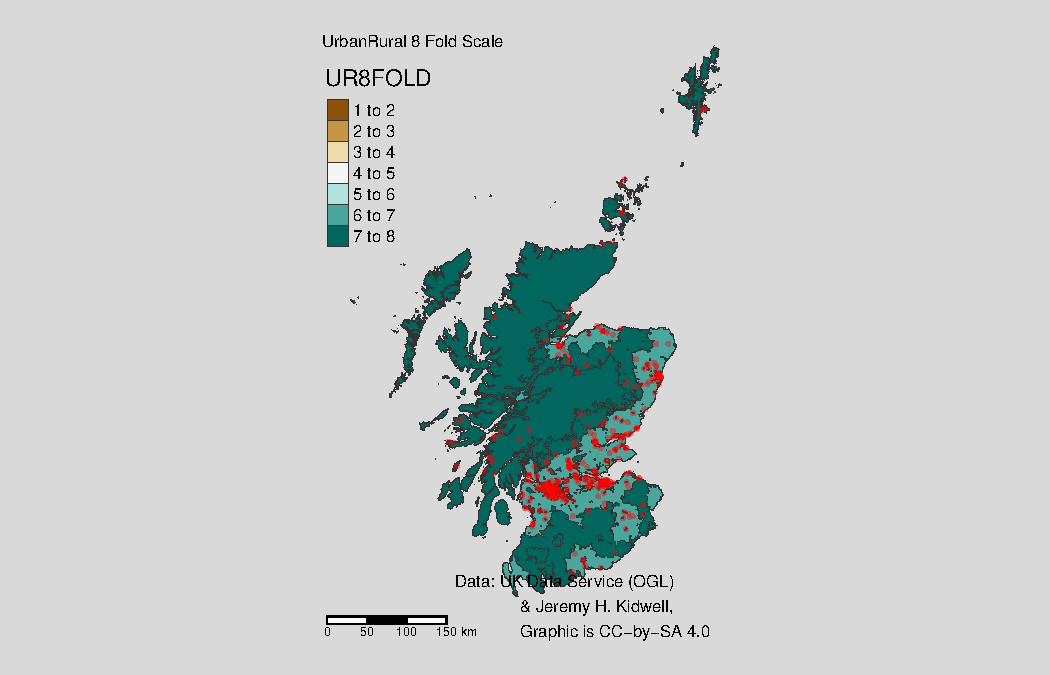
\includegraphics{figures/create_urbanrural_ecs_chart_choropleth-1.pdf}
\caption{Figure 9}
\end{figure}

\hypertarget{wealth-employment-and-literacy}{%
\section{Wealth, Employment, and
Literacy}\label{wealth-employment-and-literacy}}

\begin{verbatim}
## OGR data source with driver: ESRI Shapefile 
## Source: "/Users/jeremy/gits/mapping_environmental_action/data", layer: "sc_dz_11"
## with 6976 features
## It has 9 fields
\end{verbatim}

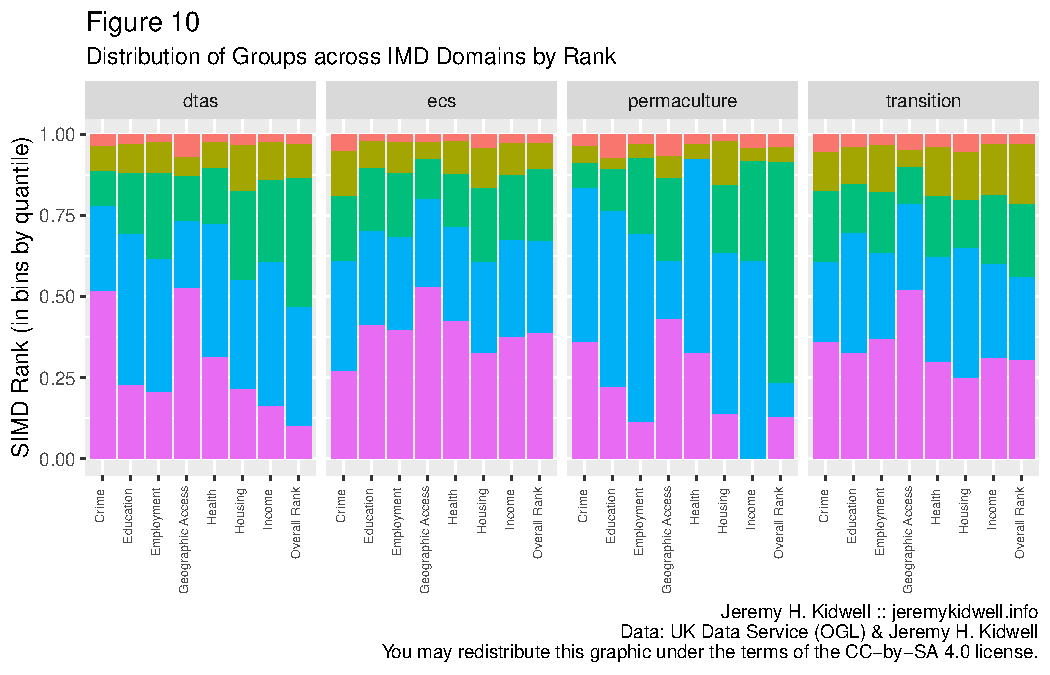
\includegraphics{figures/create_simd_barplot-1.pdf}

Another crucial point of assessment relates to the relation of
Eco-Congregation communities to the Scottish Index of Multiple
Deprivation. This instrument aggregates a large variety of factors which
can lead to deprivation including crime rates, employment levels, access
to services (implicating remoteness), and literacy. By assessing ECS,
Transition, and dtas against the deprivation scale, we can assess
whether eco-congregations fall within particular demographics and also
whether the fully aggregated SIMD measurement provides a useful point of
comparison for our purposes. The SIMD essentially divides Scotland into
6407 geographic zones and then ranks them based on their relative
deprivation. This data set can be split into any number of groups, but
for our purposes we have settled on Quintiles, splitting the SIMD data
set at every 1302 entries. We then measured where each transition group,
ECS, and dtas fell within these zones and calculated how they fell into
these five quintiles, from more to least deprived.

The first, and most compelling finding is that, in general
Eco-Congregation Scotland and Transition Scotland are both roughly the
same and match the level of population distribution in the lowest
quintile of the general SIMD measurement. 8\% of transition groups and
eco-congregation groups which have received awards and 9\% of the
population are located within this quintile. However, taken in relation
to the distribution of places of worship in the lowest quintile, we find
that eco-congregations are located at half the rate that places of
worship are (15\%) and dtass match this much more closely at 14\%.
Turning towards the top quintile, this pattern also holds, here both
transition groups (21\%) and eco-congregations (21\% and 29\% of awarded
congregations) depart from the population distribution in this upper
quintile (which is 10\%). Again, general places of worship (at 11\%) and
DTASs (at 5\%) take the opposite direction. We can say decisively that
in communities which have been identified as good candidates for
intervention to reduce deprivation, ECS and Transition are less likely,
and they are over-represented at the areas which fall into the least
deprived quintile.

We can find divergence between transition communities and
eco-congregation when we split out SIMD domains. In the lowest quartile,
measuring exclusively for the income domain, ECS is more represented
(11\%) - roughly the same as DTAS (12\%), and transition is less (6\%)
represented. In general (as shown on the chart in Appendix D), these
trends hold when representation of our groups are measured within other
non-remoteness domains of the SIMD. Our basic conclusion is that
transition towns are least likely to operate within the lowest quartile
of SIMD and DTASs are most likely, with ECS somewhere in the middle.
Given the general disparity against the presence of places of worship,
it seems fair to suggest that this might be an area for improvement,
perhaps even worth developing a special programme which might target
areas in SIMD quartile 1 for eco-congregation outreach. This might be
considered particularly in light of the starkest underrepresentation of
ECS and transition within the SIMD domain of education, skills, and
training.

\begin{verbatim}
## Reading layer `SSSI_SCOTLAND' from data source `/Users/jeremy/gits/mapping_environmental_action/data/SSSI_SCOTLAND.shp' using driver `ESRI Shapefile'
## Simple feature collection with 15872 features and 7 fields
## geometry type:  POLYGON
## dimension:      XY
## bbox:           xmin: -296506.9 ymin: 530237.9 xmax: 467721.5 ymax: 1220310
## epsg (SRID):    NA
## proj4string:    +proj=tmerc +lat_0=49 +lon_0=-2 +k=0.9996012717 +x_0=400000 +y_0=-100000 +datum=OSGB36 +units=m +no_defs
\end{verbatim}

\begin{verbatim}
## Reading layer `WILDLAND_SCOTLAND' from data source `/Users/jeremy/gits/mapping_environmental_action/data/WILDLAND_SCOTLAND.shp' using driver `ESRI Shapefile'
## Simple feature collection with 42 features and 3 fields
## geometry type:  MULTIPOLYGON
## dimension:      XY
## bbox:           xmin: 76877.24 ymin: 578454.1 xmax: 435367.1 ymax: 1190510
## epsg (SRID):    NA
## proj4string:    +proj=tmerc +lat_0=49 +lon_0=-2 +k=0.9996012717 +x_0=400000 +y_0=-100000 +datum=OSGB36 +units=m +no_defs
\end{verbatim}

\begin{verbatim}
## Reading layer `National_Forest_Inventory_Woodland_Scotland_2017' from data source `/Users/jeremy/gits/mapping_environmental_action/data/National_Forest_Inventory_Woodland_Scotland_2017.shp' using driver `ESRI Shapefile'
## Simple feature collection with 199698 features and 7 fields
## geometry type:  POLYGON
## dimension:      XY
## bbox:           xmin: 65210.1 ymin: 532547.9 xmax: 461253.7 ymax: 1209179
## epsg (SRID):    NA
## proj4string:    +proj=tmerc +lat_0=49 +lon_0=-2 +k=0.9996012717 +x_0=400000 +y_0=-100000 +datum=OSGB36 +units=m +no_defs
\end{verbatim}

\hypertarget{proximity-to-wilderness}{%
\section{Proximity to ``Wilderness''}\label{proximity-to-wilderness}}

Chasing down a curiosity, I decided to try and calculate whether
proximity to ``wilderness'' or ``scenic nature'' or just trees might
have some impact on generating more mobilised communities. I realised
that there would be several problems with this kind of calculation up
front, first being that ``nature'' is a deeply problematic construct,
reviled by geographers and philosophers alike. With this in mind, I
identified several different ways of reckoning wilderness, starting with
the highly anachronistic ``Scenic Land'' designation from the 1970s.
Then I pursued the more carefully calculated ``core wild areas''
generated by SNH just a few years ago. However, even the core wile areas
concept has been criticised heavily, so I also expanded out my search to
include all sites of special scientific interest and then went even
wider to include the Scottish Forestry Service's ``Native Woodland'' and
finally, the most generic possible measurement, any land identified as
forested at the last Forest Inventory.

Proximity to these areas was the next concern, because many of these
designations deliberately exclude human habitat, so it was necessary to
measure the number of sites within proximity. There is a question which
lies here regarding aesthetics, namely, what sort of proximity might
generate an affective connection? From my own experience, I decided upon
the distance represented by a short walk, i.e.~a half-kilometre.
However, with the more generic measurements, such as SSSI and
forestation, this wouldn't do, as there are so many of these sites that
a buffer of 500 meters encapsulates almost all of inhabited Scotland. So
for these sites I also calculated a count within 50 metres.

So what did I discover? The results were inconclusive. First, it is
important to note that on the whole, Eco-Congregations tend to be more
urban than place of worship taken generally at a rate of nearly 3:1
(5.4\% of Eco-Congregations lie in areas currently designated as ``Very
Remote Rural Areas'' whereas nearly 15\% of places of worship lie in
these areas), so what I was testing for was whether this gap was smaller
when specifying these various forms of ``wild'' remoteness. For our
narrowest measurements, there were so few sites captured as to render
measurement unreliable. There are, for obvious reasons, 0 sites located
within any of SNG's core wild areas. Similarly, there are very few of
our activist communities located within SSSI's (only
\texttt{st\_within(pow\_pointX\_sf,\ sssi)} places of worship out of
over 4k, 2 transition towns, (or 2\%) and 7 community development trusts
(3\%)). However, expanding this out makes things a bit more interesting,
within 50 metres of SSSI's in Scotland lie
\texttt{st\_within(ecs\_sf,\ st\_buffer(sssi,\ dist\ =\ 50))}
Eco-Congregations (or just under 1\%), which compares favourably with
the
\texttt{st\_within(pow\_pointX\_sf,\ st\_buffer(sssi,\ dist\ =\ 50))}
places of worship (or just 1.5\%) far exceeding our ratio (1:1.5
vs.~1:3). This is the same with our more anachronistic measure of
``scenic areas,'' there are 7 eco-congregations within these areas, and
175 places of worship, making for a ratio of nearly 1:2 (2.1\%
vs.~4.3\%). Taking our final measure, of forested areas, this is hard to
calculate, as only one Eco-Congregation lies within either native or
generally forested land.

\begin{verbatim}
## [1]  0  3 59
\end{verbatim}

\begin{verbatim}
## [1]   7  62 610
\end{verbatim}

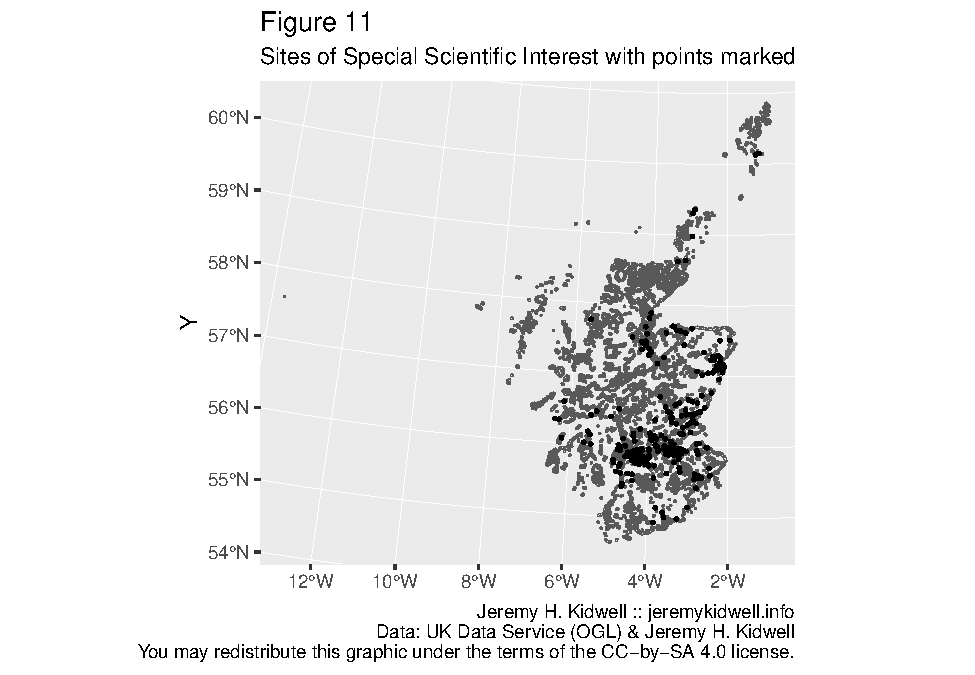
\includegraphics{figures/wilderness_plots-1.pdf}
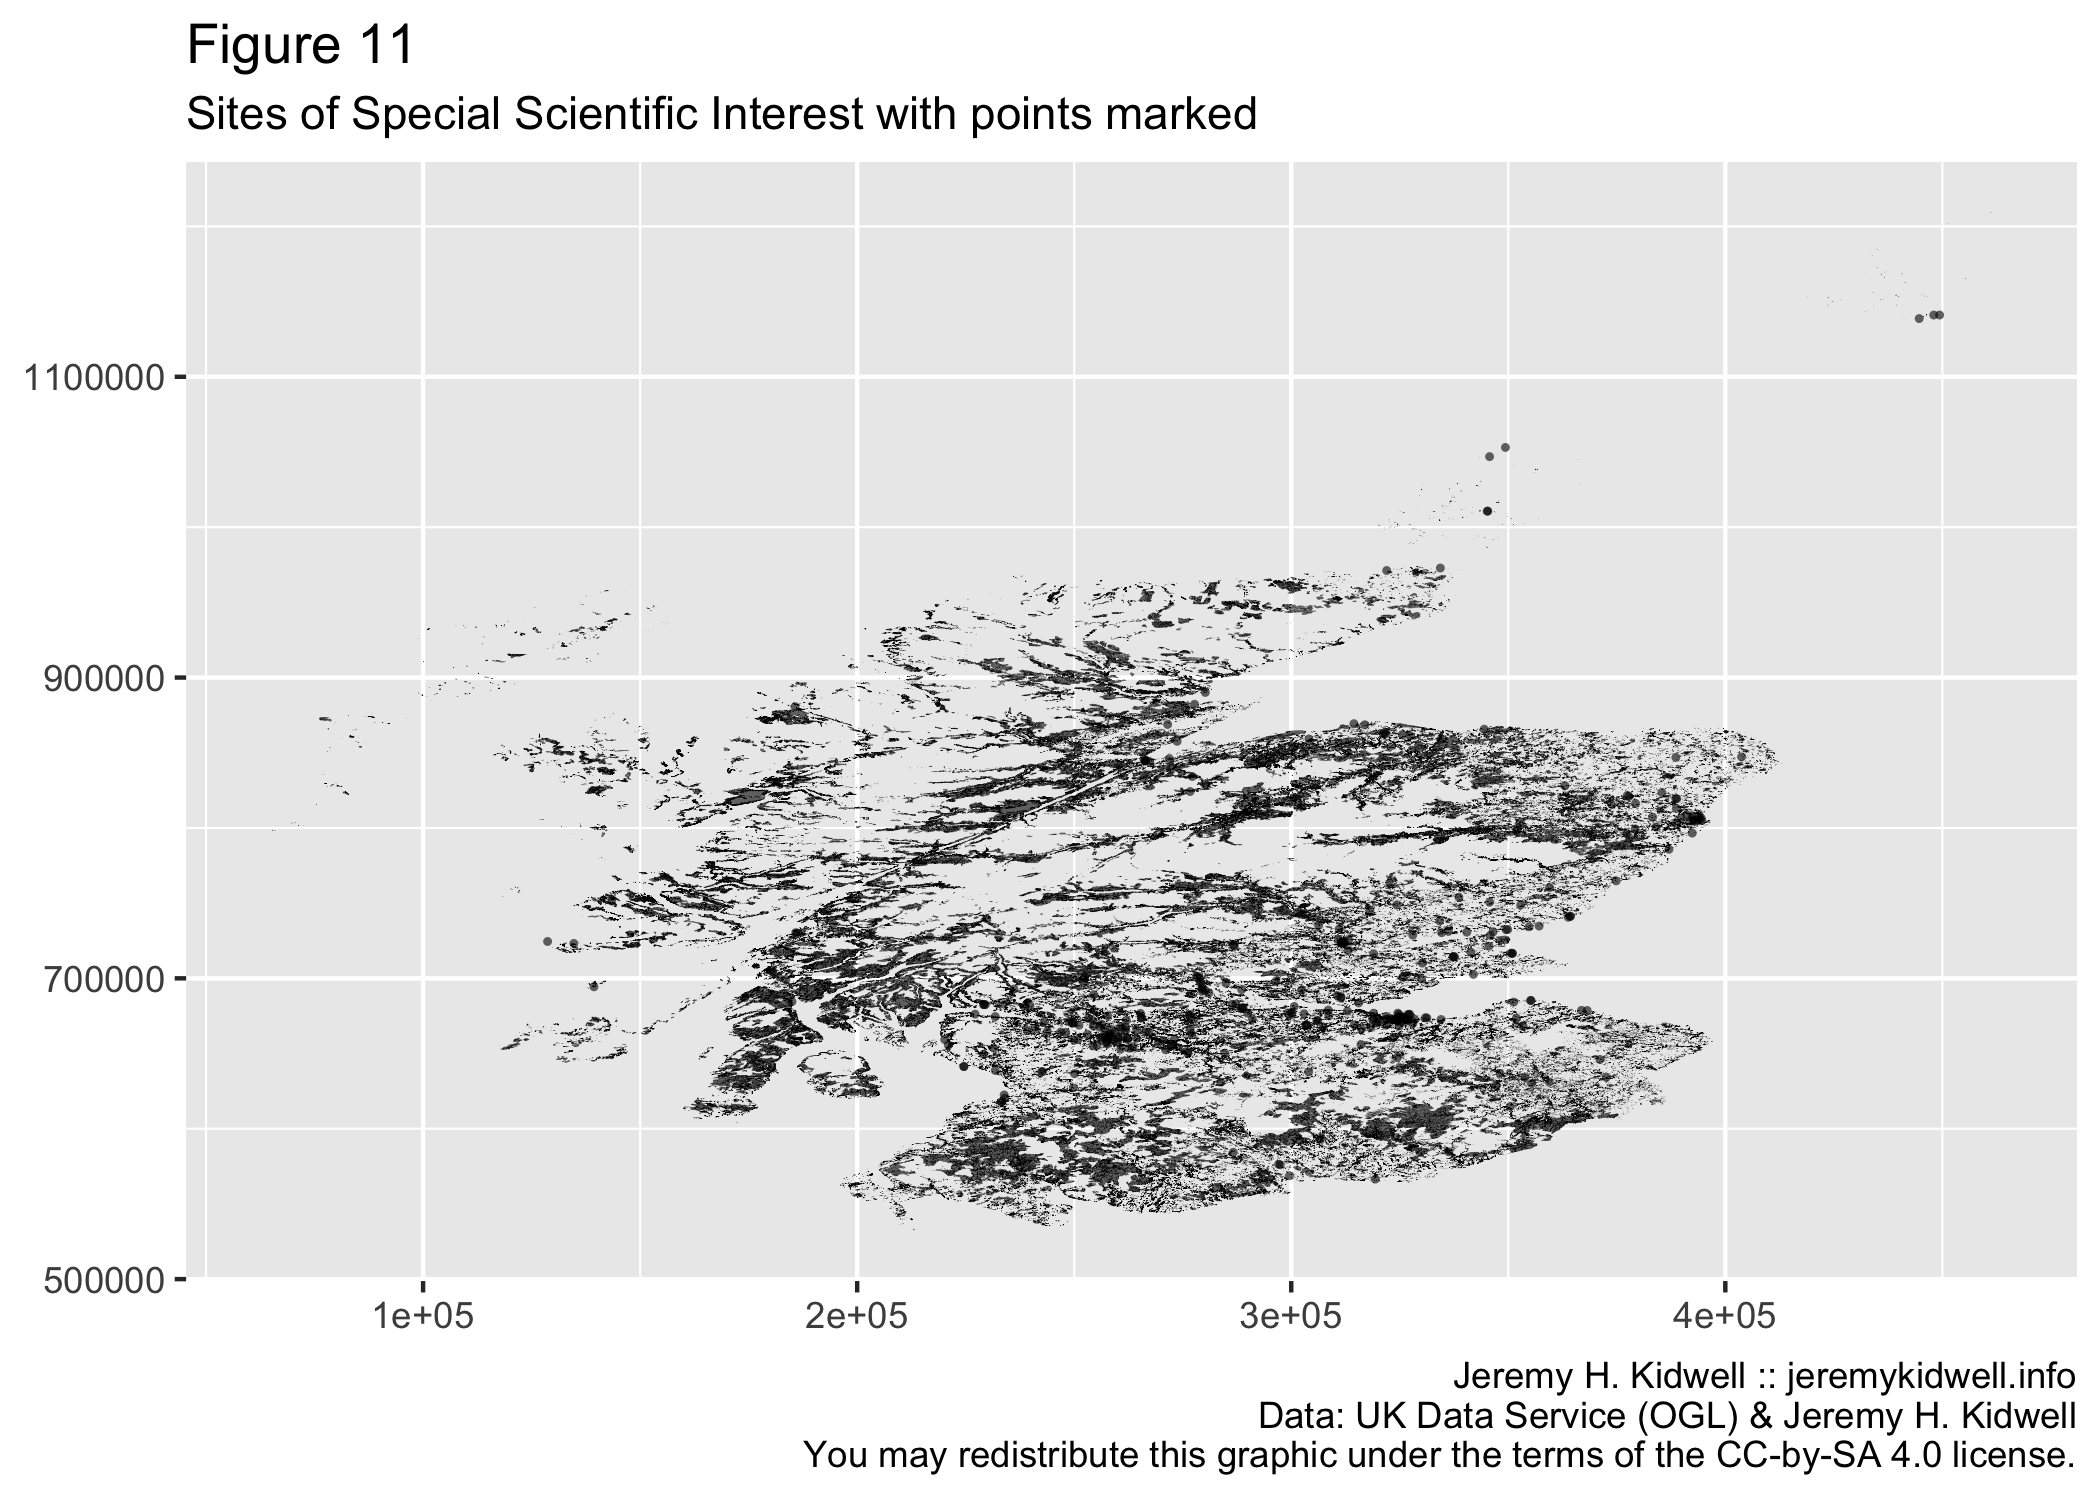
\includegraphics{figures/wilderness_plots-2.pdf}

\hypertarget{appendix-a}{%
\section{Appendix A}\label{appendix-a}}

\hypertarget{appendix-b}{%
\section{Appendix B}\label{appendix-b}}

(JK note to self: same as above, but augmented with multipliers by which
categories are different from one another)

\hypertarget{appendix-c---data-by-urban-rural-classification}{%
\section{Appendix C - Data by Urban / Rural
Classification}\label{appendix-c---data-by-urban-rural-classification}}

\renewcommand\refname{Citations}
\bibliography{biblio.bib}


\end{document}
